\documentclass[a4paper, 11pt]{article}

\usepackage[czech]{babel}
\usepackage[utf8]{inputenc}
\usepackage[T1]{fontenc}

\usepackage{graphicx}
\usepackage{float}

\usepackage[left=2cm, text={17cm, 24cm}, top=3cm]{geometry}
\usepackage{times}

\usepackage{url}
\usepackage[breaklinks,hidelinks]{hyperref}
\usepackage[hyphenbreaks]{breakurl}

\usepackage{csquotes}

\title{Dokumentace ke 2. projektu IVS}
\author{CoffeeLake}
\date{\today}



\begin{document}
	
\maketitle
\tableofcontents


\newpage

\section{Úvod}

Aplikace \emph{JCalc} je multiplatformní kalkulačka se základními funkcemi, pamětí a možností řetězit operace.\\
JCalc je licencován jako GPL3 (viz \emph{LICENCE.shtml v adresáři projektu}).

\begin{figure}[ht]
	\centering
	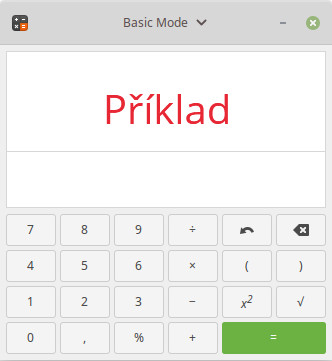
\includegraphics[width=.7\textwidth]{../screenshot.png}
\end{figure}

\section{Instalace, odinstalace programu}

\subsection{Manuální instalace}

Pro manuální instalaci budete potřebovat:

\begin{itemize}
	\item (git) (pro stažení zdrojových souborů)
	\item Gradle - vyvíjeno na verzi 5.2.1
	\item JDK - vyvíjeno na verzi 11
	\item GNU make
\end{itemize}

Postup:

\begin{enumerate}
	\item Stáhněte zdrojové soubory projektu: \emph{git clone TODO}
	\item Přejděte do složky s projektem a následně do podsložky src/
	\item Spusťte cíl \uv{jar}: \emph{make jar}
	\item pokud byl překlad úspěšný, ve složce \emph{PROJEKT/build/libs} se nachází zkompilovaný jar soubor kalkulačky
	\item Umístěte jar do složky, kde si přejete mít kalkulačku nainstalovánu (pro Windows například \emph{C:\textbackslash Program Files\textbackslash JCalc\textbackslash}, pro UNIX \emph{/opt/JCalc/}) a pojmenujte jej Calc.jar
	\item Ve stejné složce vytvořte spouštěcí skript calc.\{sh | bat\} (podle Vašeho systému) s následujícím obsahem:\\
		\subitem Pro UNIX systém:\\\\
			\emph{\#!/bin/sh\\
				java -jar Calc.jar}
		\subitem Pro Windows systém:\\\\
			\emph{java -jar Calc.jar}
			
	\item V následujícím kroku vytvořte zástupce
		\subitem pro UNIX:
			\subsubitem Vytvořte textový soubor \emph{\textasciitilde/.local/share/applications/JCalc.desktop} a zkopírujte do něj:\\\\
						\emph{
						[Desktop Entry]\\
						Type=Application\\
						Terminal=false\\
						Name=JCalc\\
						Exec=/opt/JCalc/calc.sh\\
						}

			\subsubitem Kde případně nahradíte cestu ke skriptu Vaší instalační cestou.
			
			\subsubitem Nyní byste měli najít zástupce JCalc ve spouštěči aplikací. Odtud si již jednoduše můžete umístit zástupce na plochu (konkrétní poustup je závislý na distribuci Vašeho OS, proto zde nejsou bližší instrukce)
		
		\subitem pro Windows:
			\subsubitem klikněte pravým tlačítkem na \emph{calc.bat} a zvolte \emph{Vytvořit zástupce na ploše}
			
			
	\item Pokud je aplikace funkční, můžete smazat složku se zdrojovými soubory
\end{enumerate}

\subsection{Manuální odinstalace}

Pro odinstalování proveďte následující kroky:

\begin{itemize}
	\item pro UNIX:
		\subitem Odstraňte všechny zástupce
			\subsubitem Odstraňte manuálně zástupce z plochy, pokud existuje
			\subsubitem Smažte soubor \emph{\textasciitilde/.local/share/applications/JCalc.desktop}
			\subsubitem (můžete použít příkaz \emph{rm -f \textasciitilde/.local/share/applications/JCalc.desktop})
		\subitem Odstraňte instalační složku programu. Ta je buďto \emph{/opt/JCalc}, nebo je v jiném adresáři, Vámi zvoleném během instalce
			
	\item pro Windows:
		\subitem Pokud během odstraňování podržíte klávesu Shift, soubory se rovnou odstraní, jinak se přesonou do koše
		\subitem Odstraňte všechny zástupce
			\subsubitem Odstraňte zástupce z plochy a nabídky Start (klikněte na něj pravým tlačítkem a zvolte odstranit)
		\subitem Smažte instalační složku. Ta je buďto \emph{C:\textbackslash Program Files\textbackslash JCalc}, nebo je v jiném adresáři, Vámi zvoleném během instalce
\end{itemize}

\section{Jak pracovat s programem}

\section{Závěr}

Vytvořili\\Marek Lohn,\\René Szotkowski a\\Ondřej Mikula\\\\jako projekt v předmětu IVS.\\\\
FIT VUT, Brno, 2020.

\end{document}